\chapter{绪论}
\label{chapter:intro}

\section{研究背景}
\label{section:background}

生物信息学是研究生物信息的采集、处理、存储、传播和解释等各方面的学科。
生物信息学可以帮助人类从海量的生物数据中挖掘内部的生理过程规律,从而指导进一步的生物学研究。在规模化实验大力发展和海量数据爆发的如今,如何有效的利用生物数据变得越来越中了。
生物信息学分为三个主要的发展阶段,前基因组时代主要建立了各种生物数据库和序列比较算法、基因组时代进行了大规模的基因测序以及目前所处的后基因组时代。
后基因组时代研究重心以生物数据分析为主,并且挖掘的层次逐渐深入。已经从对基因组直接的结构的研究逐渐转向对基因功能的研究,其中的主要侧重点包括基因组学、转录组学以及蛋白质组学等\cite{helms_principles_2019}。

蛋白质是生物细胞和组织的重要组成部分,是生命体的物质基础,也是遗传信息的直接表达手段,涉及生物体载体、免疫、激素等方方面面。蛋白质分子深度参与了组织的构成与修复、生理功能的调节和能量的供给。
蛋白质组学\cite{schubert_quantitative_2017}是在蛋白质表达层面研究生理生化功能为主的一门学科,目的是揭示蛋白质的基本生命活动规律,其中研究主要关注蛋白质结构、蛋白质丰度、蛋白质修饰以及蛋白质相互作用。

蛋自质在细胞活动中发挥着巨大的作用。但是在多数情况下单个蛋自质无法独立的执行生物功能,只有构成蛋白质复合物,才能有效的参与到细胞活动中\cite{gavin_functional_2002}。因此蛋白质复合物的结构、功能及形成方式的研究就显得尤为重要。图\ref{fig:swr1_complex}是具有染色质重塑功能的酵母SWR1复合物。
\begin{figure}[htbp]
  \centering
  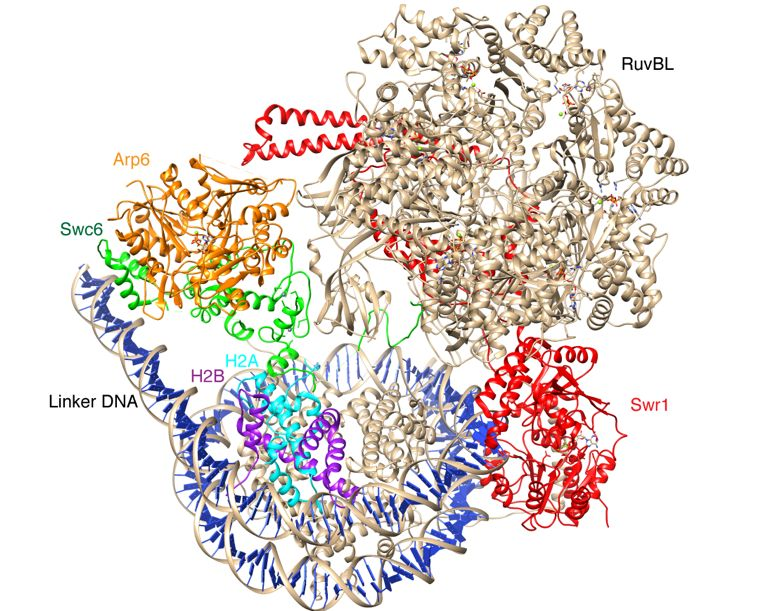
\includegraphics{SWR1_complex}
  \caption{酵母菌SWR1复合物}
  \label{fig:swr1_complex}
\end{figure}
生物实验中检测蛋白质复合物主要通过串联亲和纯化与质谱分析\cite{g_generic_1999}、酵母双杂交\cite{li_identification_1993}两种技术对蛋白质复合物进行分离和鉴定。串联亲和纯化与质谱分析通过靶蛋白标定以及自然条件下亲和纯化获取可能的蛋白质复合物,再使用质谱分析进行鉴定。酵母双杂交技术利用转录调控因子中的组件特征研究蛋白质之间的相互作用关系。虽然基于实验测定的方法具有生物学上的可解释性,但是生物实验往往条件困难、实验步骤多且成本昂贵,无法满足快速增长的研究需求。

蛋白质与生理环境存在广泛的相互作用,蛋白质复杂功能的实现同蛋白质之间、DNA与蛋白质、RNA与蛋白质的相互作用密切相关,蛋白质复合物正是一组强相关的蛋白质组合共同作用的结果。随着生物信息学的发展以及高通量技术的发展,蛋白质相互作用关系(Protein-ProteinInteraction,$PPI$,后简称为互作关系)得到了大量的补充,促成了大规模互作网络的构建\cite{butland_interaction_2005},即蛋白质相互作用网络(Protein-ProteinInteractionNetwork,$PIN$)。图\ref{fig:ppi}为酵母菌蛋白质相互作用网络。
\begin{figure}[htbp]
  \centering
  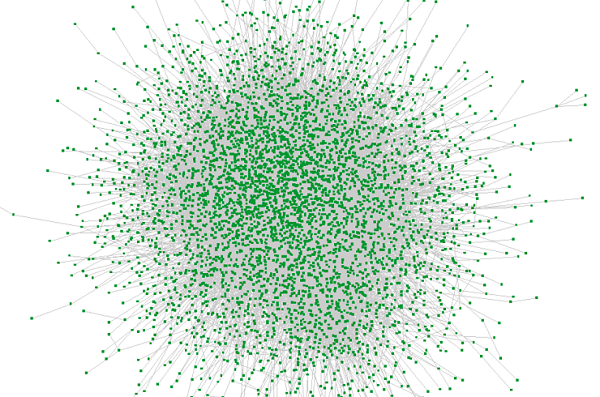
\includegraphics{ppi}
  \caption{酵母菌蛋白质相互作用网络}
  \label{fig:ppi}
\end{figure}
已知的蛋白质复合物可以视作互作网络里面的一系列子网络,因此利用图论和计算模型学习子网络的分布模式,即可在互作网络中发掘潜在的蛋白质复合物\cite{legrain_proteinprotein_2001}。利用图论的方法,蛋白质互作网络可以转换为无向图~$G=(V,E)$。其中$V$为图中结点的集合,表示所有的蛋白质,$E$为图中邻边的集合,表示所有的蛋白质互作关系。$PIN$转换为图结构之后,图论上的计算模型和深度学习方法就可以迁移到蛋白质复合物的研究中。2002年,Tong\cite{tong_combined_2002}等人提出了密集子图的假说,蛋白质复合物在$PIN$是密集链接的子图,而与其他的蛋白质连接相对稀疏。在$PIN$中预测蛋白质复合物的问题就转换为了密集子图的挖掘问题,逐渐发展出了利用$PIN$和计算方法识别蛋白质复合物的理论。

\section{国内外研究现状}
\label{section:research}

现有的基于计算方法的蛋白质复合物预测方法主要分为五类:基于网络结构的图聚类方法、融合生物信息的图聚类方法、核心附属扩展方法、动态网络方法以及监督学习方法。以下分别对这五类方法的研究现状做简单的介绍。

\subsection{基于网络结构的图聚类方法}
\label{section:TopologyMethod}

MCODE算法\cite{bader_automated_2003}是最早提出基于网络结构构造密集子图的复合物预测算法。首先算法会计算所有结点的局部邻居密度,其中密度超过平均值的结点成为种子,视作初始子图。满足相应阈值条件的邻居结点不断扩充子图,直到阈值条件饱和,最终子图视为预测的复合物,算法最终会过滤掉结点数少的复合物。Clique算法\cite{spirin_protein_2003}通过穷举法、超顺磁性聚类和蒙特卡洛模拟三种方法搜索完全图来检测蛋白质复合物。RNSC算法\cite{king_protein_2004}以随机聚簇最为初始聚簇,按照代价函数逐渐削减聚簇,最终形成蛋白质复合物。马尔科夫聚类算{}也被应用于蛋白质复合物的检测,例如Pereira-leal等人9提出的方法。马尔科夫聚类算法通过膨胀及扩展操作实现在蛋白质相互作用网络上计算概率转移矩阵以及搜索连接紧密的蛋白质子图以预测蛋白质复合物。扩展操作是通过转移矩阵的不断自乘来连接图的不连通区域。膨胀操作通过计算矩阵内元素的幂来增大当前的大概率,减小当前的小概率。重复进行膨胀、扩展操作,最后获得蛋白质复合物。L等人10提出的LCMA算法,首先找到蛋白质相互作用网络中较小的完全图,然后通过合并重合率高的完全图,从而检测蛋白质复合物。CFinder算法1采用派系过滤算法(ClusterPercolationMethod,简称CPM)[12],通过完成k阶完全图的搜索和相邻阶完全图的合并这两个主要步骤来实现蛋白质相互作用网络中的蛋白质复合物预测。所谓k阶完全图的相邻是指网络中个k阶完全图存在k-1个公共节点,则这两个阶完全图相邻。SCAN算法3]公共邻居数大于给定阈值的两个蛋白质认为是结构可达的,以结构可达节点最多的节点作为种子节点向外扩展逐步将结构可达的邻居节点纳入聚簇。ClusterONE算法4是Nepusz等人提出的,基于蛋白质聚簇内部节点连接紧密、聚簇内部与外部节点连接稀疏的特性,重新定义了子图紧密性的概念。主要思路是利节点度的大小完成排序及向外扩展操过程,通过添加或删除节点,使得子图紧密最优。重复以上步骤,直到遍历所有节点,以此预测出重叠的蛋白质复合物。Zhang等人1提出根据子图中三节点连通图的个数来定义局部子图连紧密性,然后采用与ClusterONE近似方法,从节点度数最大的节点开始向外扩展,通过增加或删除节点,使得子图紧密度最大。Zheng等人提出GAGC算法,基于遗传算法检测蛋白质复合物。个体对应于聚类结果,F1值对应于种群进化的适应度函数除了由局部密集子图引申出来的一系列预测算法,通过对已知复合物的内部结构特征的具体研究发现大多数蛋白质复合物都遵循核心附属结构,也就是说,蛋白质复合物由核心蛋白质和附属蛋白质两部分组成,如图1.4所示。核心蛋白质是指存在大量相互作用的蛋白质集合,而相对稀疏的其他蛋白质构成附属蛋白质集合。
Leung等人17提出的CORE算法通过两个蛋白质与公共邻居的相互作用数来计算其属于同一个复合物核心蛋白质的概率。之后,通过不断合并小的核心蛋白质集合以得到用以扩张的核心蛋白质,再根据其他节点与核心节点(即核心蛋白质)的连接强度大小,添加附属蛋白质,最终构成蛋白质复合物。Wu等人提出的COACH算法根据复合物的核心附属结构模型预测复合物。网络中
\subsection{融合生物信息的图聚类方法}
\label{section:appendBiology}
\subsection{核心附属扩展方法}
\label{section:CoreAppend}
\subsection{动态网络方法}
\label{section:Dynamic}
\subsection{监督学习方法}
\label{section:Supervision}
\subsection{方法总结}
\label{section:researchSummary}

\section{研究动机和思路}
\label{section:motivation}

国内外学者对复合物的识别已经提出了诸多方法,总体趋势也是趋向于融合生物数据和网络数据并达到更精确的预测,但是目前现有的方法还存在以下的不足。
\begin{itemize}
  \item上述的研究方法主要是基于无监督方法,无法利用到已有的蛋白质复合物信息。
  \item部分模型方法如{}本质上是一种基于随机性的方法,这类方法为了达到较高的召回率,往往倾向于产生过量的候选复合物,这样往往导致结果的准确率的降低。
  \item没有有效的融合生物信息
\end{itemize}

\section{论文组织}
\label{section:organization}